\chapter{Обзор} \label{chapt1}

\section{Ситуативный анализ засухи} \label{sect1_1}


Республика Узбекистан расположена в центральной части Евроазиатского континента. Ландшафт Узбекистана разнообразен по формам рельефа - это плато, низменные и подгорные равнины (70\%), отроги гор и горные хребты (20\%). Почти 80\% площади страны занимают пустыни и полупустыни, включая крупнейшую пустыню Центральной Азии – Кызылкум. 
Климат Узбекистана - резко континентальный, засушливый, для него характерно обилие тепла и света. По индексу аридности ЮНЕП (от 0,05-0,20 до 0,65) территория страны (за исключением предгорной и горной части) относится к засушливой зоне, находящейся под угрозой воздействия атмосферной (воздушной) и почвенной засух и, соответственно, уязвима к процессам деградации и опустынивания \cite{Zasuha2013}.

Существует не одно понятие и тип засухи, в целом \textit{\textbf{засуха}} — продолжительный (от нескольких недель до двух-трёх месяцев) период устойчивой погоды с высокими для данной местности температурами воздуха и малым количеством осадков (дождя), в результате чего снижаются влагозапасы почвы и возникает угнетение и гибель растений.
Засуха - это явление характерное для Узбекистана, часто повторяющееся, масштабное по охвату территории и, соответственно, затрагивающее практически все слои населения. Оно является доминирующим среди других природных бедствий в Узбекистане \cite{Agalceva2012, Zasuha2005, Chub2007}. Доля населения, проживающего в районах, подверженных засухе составляет 76,3\% \cite{Zasuha2013}. Засуха отрицательно влияет на экологическое состояние природной среды, наносит существенный ущерб экономике страны и отражается на благосостоянии населения. Согласно проведенным оценкам наиболее уязвимым сектором экономики Узбекистана по отношению к засухе является сельское хозяйство. Поэтому, сегодня особо актуальными являются вопросы мониторинга, предупреждения и готовности к засухе с целью смягчения ее негативных последствий. 

\subsection{Типы засухи}

Для Узбекистана характерна засуха четырех видов:
\begin{enumerate}
	\item метеорологическая,
	\item гидрологическая,
	\item почвенная засуха,
	\item сельскохозяйственная.
\end{enumerate}

Атмосферная или метеорологическая засуха характеризуется длительным и значительным недостатком осадков по сравнению с долгосрочными средними показателями, при повышенных температурах воздуха в вегетационный период (весной или летом) и обуславливает высокие значения транспирации и испарения.

Гидрологическая засуха- дефицит водных ресурсов поверхностного или подповерхностного стока в результате недостатка осадков \cite{Chub2001}. По определению ВМО «Гидрологическая засуха - достаточно продолжительный период сухой погоды, вызывающий недостаток воды в результате понижения расхода ниже нормы и/или понижение содержания влаги в почве и уровня грунтовых вод». Этот вид засухи является особо опасной угрозой для развития страны.

Почвенная засуха – иссушение почвы, связанное с атмосферной засухой, то есть с определенными условиями погоды в вегетационный период, что вызывает недостаточное водообеспечение растительности и сельскохозяйственных культур, их угнетение и снижение или гибель урожая. 

Сельскохозяйственная засуха связывает различные характеристики засухи с воздействием на сельское хозяйство, фокусируясь на дефиците осадков, различиях между фактической и потенциальной эвапотранспирацией, дефиците воды в почве, понижение уровня грунтовых вод.
При засухе поступление воды в растения через корневые системы затрудняется, расход влаги на транспирацию начинает превосходить её приток из почвы, водонасыщенность тканей падает, нормальные условия фотосинтеза и углеродного питания нарушаются.

При засухе поступление воды в растения через корневые системы затрудняется, расход влаги на транспирацию начинает превосходить её приток из почвы, водонасыщенность тканей падает, нормальные условия фотосинтеза и углеродного питания нарушаются.
Необходимо отметить, что в зависимости от времени года различают весенние, летние и осенние засухи: 
\begin{enumerate}
	\item весенние засухи особенно опасны для ранних зерновых культур,
	\item летние причиняют сильный вред как ранним, так и поздним зерновым и другим однолетним культурам, а также плодовым растениям,
	\item осенние опасны для всходов озимых.
\end{enumerate}

Все виды засух приводят к негативным социальным, экономическим и экологическим последствиям. На рисунке \ref{img_drought_types} показано взаимодействие типов засухи, их продолжительность и влияние на экономические, экологические показатели \cite{PROON2012}.

\begin{figure}[ht] 
	\centering
	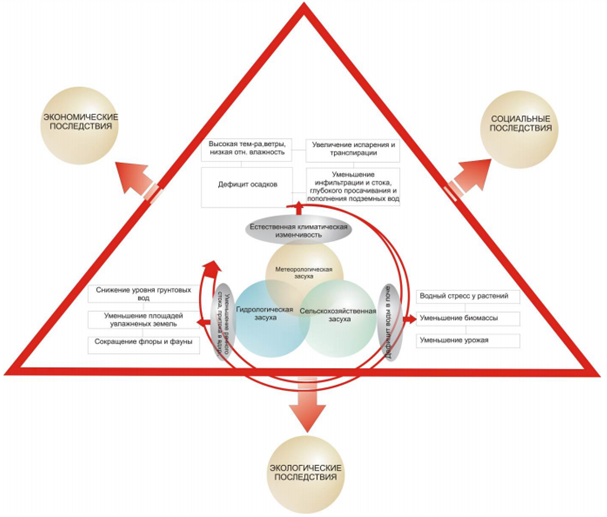
\includegraphics [scale=0.7] {drought_types}
	\caption{Виды засухи, их взаимодействие и влияние \cite{PROON2012}.}
	\label{img_drought_types}
\end{figure}

Засушливые явления отличаются друг от друга по трем основным характеристикам: интенсивность, продолжительность, пространственный охват. 

Они сопровождается высокими температурами воздуха при малом количестве осадков. Температура, равная и выше 35 \textdegree С, наблюдается в стране, преимущественно, с конца мая по октябрь, хотя в отдельные годы, особенно на юге, жара начинается уже в апреле, а иногда даже в марте. Пик числа жарких дней приходится в среднем на июль, хотя в отдельные годы наблюдается и в августе месяце. Почвенная засуха наблюдается в пустыне Кызылкум и Центральной Фергане с конца марта или начала апреля. На равнинных территориях этот процесс начинается с первой декады апреля, а в восточной части страны и предгорьях - в июле месяце \cite{Chub2001, Chub2007}.

В предгорной зоне Узбекистана очень сильная засуха (SPI < -50) весной наблюдается редко - 1--3 раза за 100 лет, а засуха с дефицитом сезонных сумм осадков в 20--25\% (SPI < -20) является достаточно регулярным явлением, наблюдаемым с вероятностью 30\%. 
В зоне пустынь и полупустынь очень сильная весенняя засуха (SPI < -50) проявляется в среднем 1 раз в 10 лет. Число дней с атмосферной засухой на большей части равнинных ландшафтов не превышает 30 дней, на юге эта цифра возрастает до 30-50 дней, и в Каршинской степи достигает 50-70 дней \cite{Chub2007}. Сравнительный анализ значений индекса осадков SPI с индексом по снегозапасам для зимних осадков (январь-март) и стоком за вегетацию в бассейнах рек Ахангаран и Пскем подтверждает определенную синхронность их колебаний.

В последнее десятилетие наблюдается увеличение периодичности засухи - она становится более частой в летний и осенний сезоны, особенно в низовьях реки Амударьи и в окрестностях Аральского моря. В 80-х и 90-х годах прошлого столетия засуха наблюдалась в среднем 2 раза в 10 лет. За период 2000 -- 2012 гг экстремальная засуха была зафиксирована 4 раза - в 2000, 2001, 2008 и 2011 годах []. 

Суровая засуха 2000-2001 годов стала особо опасной по масштабам распространения, воздействиям и последствиям для сельского и водного хозяйства и других секторов экономики, окружающей среды и сельского населения. Ответные меры и уроки, полученные в период суровой засухи 2000-2001гг, были детально изучены всеми заинтересованными учреждениями и международными организациями \cite{Zasuha2005}.
По данным \cite{Agalceva2012} 2011 год стал экстремально засушливым годом для Узбекистана за прошедшие 60 лет. Практически по всей территории Узбекистана наблюдается увеличение числа дней с температурой 40 \textdegree С и более, по сравнению с среднемноголетними данными. Это подтверждает тренд долгосрочных изменений показателей метеорологической и гидрологической засухи в бассейне реки Кашкадарья (пост Варганза) за период 1960-2011 гг. На значительной части Узбекистана было зафиксировано число засушливых дней с дефицитом влажности воздуха E $\geq$ 50 гПа в пределах нормы и выше нормы. Согласно прогнозным оценкам подобные тенденции, станут более широко распространенными \cite{NatSoob2, NatSoob3}.

Участившиеся засухи причиняют огромный ущерб и несут угрозу для жизнедеятельности населения, безопасности и социально-экономического развития страны. Воздействия засухи затрагивают практически все сектора экономики и сегменты населения, и представляют реальную угрозу благосостоянию населения и продовольственной безопасности Республики.
Биофизические воздействия. Из-за природно-географических и климатических особенностей Узбекистан очень чувствителен к деградации природной среды, особенно в связи с хрупкостью аридных систем и ограниченностью водных ресурсов. 
Засухи снижают буферные и фильтрационные свойства почвы, ее роль в гидрологическом и азотном циклах, способность обеспечить среду обитания для микроорганизмов и поддерживать биоразнообразие. Потеря растительного покрова вызывает сильную эрозию почв, уплотнение структуры почв и потерю здоровья почв. Засуха усиливает мобилизацию и аккумуляцию солей в верхних горизонтах почв и увеличивает засоление и деградацию земли во времени и в пространстве \cite{Zasuha2013}.

Засуха снижает доступность пастбищ для домашнего скота и диких животных. Численность диких пастбищ также имеет тенденцию к сокращению в связи с миграцией животных и потерей биомассы, которые возникают от недостатка воды. 
Более частые атмосферные засухи, с экстремально высокими температурами и низкой влажностью, особенно опасны в сочетании с недостатком воды для орошаемого земледелия - происходит угнетение посевов, недобор и/или гибель урожая на больших территориях. Например, потери урожая зерновых культур в годы суровой засухи 2000-2001 составили 14-17\%, а по другим культурам - в среднем от 45- 52\% до 75\% (низовья Амударьи).

Фактически, засуха 2000-2001гг формировалась постепенно, была необычной из-за дефицита осадков в сочетании с высокими уровнями испарения, вызванными жаркой погодой в течение нескольких лет. Уровни осадков достигли лишь 40\%-60\% от нормы, что привело к чрезвычайному сокращению речного стока (на 35\%-40\% от среднего уровня). Речной сток в низовье р. Амударьи был рекордно низким - Каракалпакстан получил лишь 20-30\% от потребности воды в период вегетации 2000 года. Гидрологические и социально-экономические эффекты засухи ощущались до конца 2003 года, в то время как осадки и сельскохозяйственное производство возвратились в норму в большинстве районов в 2002 г. \cite{Zasuha2013}.

Засуха 2000-2001гг. явилась катализатором процессов опустынивания и деградации окружающей среды, особенно в низовьях реки Амударьи. К концу 2001 г. практически полностью пересохли озерные системы озер и ветланды в северной части Каракалпакстана, площадью около 160 тыс.га. В результате исчезновения водно-болотной среды обитания в Красную книгу Узбекистана в 2000-2001 гг. было занесено 46 видов. Уровень подземных вод в районах охваченных засухой снизился до 10-15 метров, в результате большинство артезианских колодцев оказались бесполезными. Ухудшилось качество воды - минерализация воды в реки Амударья (Каракалпакстан) составила 0.85-2.1 г/л, жесткость достигала 17 мг/л.

Социально-экономические воздействия. Экономические и социальные воздействия засухи являются существенными и многоплановыми и проявляются, в частности, в сокращении сельскохозяйственной продукции и увеличении масштабов малообеспеченности, нехватке продовольствия и воды для хозяйственно-бытовых и питьевых нужд, росте детской смертности и обострении социальных конфликтов и/или усилении экологической миграции.

Нарушение динамики и производительности услуг напрямую влияют на продуктивность растениеводства, животноводства и рыбоводства и отвлекает значительные финансовые ресурсы страны на ликвидацию последствий в пострадавших регионах и т.д. Полный анализ издержек усложнен неопределенностью границ, поэтому во многих случаях зачастую не учитываются косвенные потери, издержки за пределами затрагиваемого района или соотношение издержек в случае осуществления действий и в случае бездействия. Соответственно, потенциальные экономические выгоды сокращения масштабов засух часто сильно недооцениваются.

Анализ последствий засухи 2000-2001 гг., по Каракалпакстану и Хорезмской области показывает, что наиболее драматические снижения в сельскохозяйственном производстве происходили вследствие недостаточности планирования, прогнозирования и контроля над водными ресурсами на региональном, республиканском и местном уровнях, что привело к уменьшению водоподачи на 20-30\% и 35-80\% соответственно по сравнению с утвержденным лимитом на воду. Как следствие, около 200 тыс. хозяйств (1.000.000 человек) потеряли урожаи.

По данным регионального обзора убытки, вызванные сельскохозяйственной засухой 2000-2001гг. в Узбекистане составили 130 млн. долларов США или 2.4\% от с/х ВВП. По другим источникам \cite{Zasuha2013}, величина ущерба оценивается в размере 38-40 млн. долларов США.
Значительные потери отмечались в животноводческом секторе. Чрезмерно стравленные пастбища вокруг сельских населенных пунктов и кишлаков были полностью лишены водоснабжения. В результате, заготовка кормовых трав сократилась более, чем на половину. В некоторых затронутых районах Каракалпакстана, засуха вынудила фермеров продать значительную часть своего стада или сельскохозяйственного оборудования.

Потеря биопродуктивности биоценозов и водной биоты водоемов в результате критических изменений гидрорежима в дельте Амударьи в годы засухи привели к тотальной гибели популяций промысловых рыб региона, подрыву ресурсной базы и краху рыбного хозяйства. За всю историю рыболовства наименьший улов рыбы в дельте Амударьи был в последующие после засухи годы: 131.6 тонн (2003) и 239.2 тонны (2004). На грани банкротства оказалось 51 фермерских хозяйств Каракалпакстана, арендовавшие свыше 60 тыс. га озерных систем.

Помимо экономического ущерба, засуха оказала значительные социальные эффекты. Наиболее сильно пострадавшему населению (порядка 600 000 человек) потребовались продукты питания, питьевая вода, помощь в поставке сельхозресурсов, затраты на которые в 2000-2001 гг. в Узбекистане составили 19 млн. долларов США. Оценки показали, что 2001 года порядка 79 000 хозяйств в Каракалпакстане и 21 000 в Хорезме остались без работы. Увеличилась миграция за пределы Узбекистана (в основном из Каракалпакстана в Казахстан) в поисках лучших жизненных условий. 
Недостаток воды для полива и/или ее низкое качество приводит к тому, что на всех уровнях (особенно домохозяйств и фермеров) происходит поиск адекватных стратегий преодоления нехватки воды. Это поиск дополнительных источников воды, меры по водосбережению и улучшению ирригационной и дренажной сети, и другие виды деятельности. Все они требуют труда, энергии, материальных затрат и навыков, но также влекут за собой социальные и экологические риски. В большинстве случаев, не имея альтернативных источников воды, усилия фермеров и дехкан сводятся к отбору воды из коллекторов и/или подземных вод, что вызывает засоление и деградацию земли, и связанные с этим ущербы урожая и, другие экономические и экологические ущербы. Ненадежная подача воды на орошение и ухудшение земли (особенно, засоление и заболачивание участков) усугубляют проблемы малообеспеченности.

В последнее десятилетие инвестиции и вклады государства при поддержке международных организаций в водный и сельскохозяйственный сектора и рост занятости в несельскохозяйствен¬ной сфере, способствовали диверсификации сельского хозяйства, предоставляя фермерам и пастухам более широкие возможности для преодоления засухи и смягчения ее эффектов. Тем не менее, большинству фермеров не хватало средств и знаний, чтобы воспользоваться преимуществами доступа к информации и смягчающим мерам, а развитие занятости в несельскохозяйственном секторе значительно отставало от других инициатив в области сельскохозяйственного развития.

Согласно данным опроса общественности, проведенного Центром социологических и рыночных исследованиям «Эксперт Фикри», в районах, пострадавших от засухи 2000-2001 гг., в результате недостатка воды участились случаи диареи и кишечных расстройств, острых респираторных заболеваний и болезней, связанных с употреблением некачественной воды. 

Меры по смягчению последствий засухи, как правило, осуществляются в порядке реагирования с точки зрения управления действиями в кризисных ситуациях и, как известно, такое реагирование не приносит должного результата. В годы засух создается специальная Комиссия с привлечением всех ключевых министерств и ведомств, которая разрабатывает меры и действия по смягчению последствий засухи \cite{Zasuha2013}. 

\subsection{Мониторинг и оценка}
Выбор индикаторов засухи является одним из главных вопросов организации мониторинга и оценки засух. 
Основу мониторинга засухи составляют данные наблюдений за метеорологическими, гидрологическими и агрометеорологическими параметрами - характеризующими частоту, пространственное распределение и продолжительность засух, которые проводит Узгидромет. 
Сеть наземных наблюдений включает: 
\begin{enumerate}
	\item 130 – гидрологических постов; 
	\item 79 – метеорологических станций на ежедневной и десятидневной основе; 
	\item агрометеорологические наблюдения, которые ведутся на 61 станции и 30 постах; 
	\item наблюдения за состоянием снежного покрова на 12 наземных и 138 аэровизуальных пунктах. 
\end{enumerate}

Помимо наземного мониторинга для оценки и предупреждения засух применяются данные дистанционного зондирования земли.
Перечень данных необходимых для предупреждения и оценки засух.

\begin{enumerate}
	\item Метеорологическая засуха 

	\begin{enumerate}
		\item Временной ряд климатических показателей, влияющих на засуху: температура, влажность воздуха, потенциальная эвапотранспирация;
		\item Частота засушливых лет;
		\item Прогнозируемая частота засушливых лет при различных сценариях климатических изменений;
		\item Количество и состояние метеорологических станций.
	\end{enumerate}

	\item Гидрологическая засуха

	\begin{enumerate}
		\item Временной ряд данных о площади и объеме поверхностных вод, сборе, подземных водных ресурсах, инфильтрации и изменчивости водного горизонта;
		\item Временной ряд данных о водном балансе: планируемые и фактические заборы воды различными отраслями; процентная доля ВВП и занятости в различных секторах;
		\item Временной ряд данные по областям и районам по орошаемым и не орошаемым участкам (планируемый и фактический), водозаборы для этих участков, и потери воды в магистральных каналах и в межхозяйственных и внутрихозяйственных ирригационных системах;
		\item Частота гидрологической засухи (разной степени) в разных районах;
		\item Количество и состояние станций по мониторингу стока и снежного покрова
		\item Меры по водоуправлению, за последние 10-15 лет, на межгосударственном и местном уровнях, такие как проведение переговоров, регулирование водохранилищ, сокращение лимитов, планы по водопользованию, ротации и т.д.;
		\item Минимальная/максимальная потребность гидроэнергетического потока и наличие водных ресурсов; процент электричества, генерируемого гидроэнергетикой;
		\item Максимальная/минимальная потребность воды для рыбного хозяйства и наличие водных ресурсов; оцениваемые потери;
		\item Максимальная/минимальная потребность воды для ветландов и экологическая сбалансированность рек и наличие водных ресурсов;
		\item Воздействие гидрологической засухи на опустынивание;
		\item Уязвимость.
	\end{enumerate}

	\item Сельскохозяйственная засуха

	\begin{enumerate}
		\item Количество и состояние агрометеорологических станций;
		\item Зависимость урожая от погоды (орошаемые и неорошаемые угодья, пастбища);
		\item Качество почв в основных агроэкологических зонах; классификация состава, содержание гумуса, способность почвы удерживать влагу, бонитет;
		\item Процентная доля орошаемых и неорошаемых земель в ВВП и т.п.;
		\item Диверсификация производства (растениеводство, животноводство, агролесоводство и т.п.);
		\item Процентная доля посевных земель, садов и пастбищных орошаемых ресурсов;
		\item Процент засоленных почв различной категории;
		\item Реагирование урожая на засоление воды и/или почвы, при различных культурах;
		\item Скотоемкость пастбища, процент деградированных пастбищ, максимальный погектарный выпас скота по регионам;
		\item Структуры земледелия и оцененные потребности в воде;
		\item Внутрихозяйственные агротехнические меры, предпринимаемые во врем и после засухи;
		\item Урожайность культур по районам;
		\item Ущерб от засух
	\end{enumerate}
\end{enumerate}

\subsection{Подходы и методы оценки засухи. Предупреждения засухи}

Засухи из опасных гидрометеорологических явлений являются наиболее дорого обходящихся природных опасных явлений, т.к оказывают значительные воздействия одновременно на многие сектора экономики и население. Но медленное наступление засухи дает потенциальную возможность к ее управлению. 

Управление засухой должно учитывать постоянное наблюдение и оценку состояния за определенными показателями/индикаторами засухи, оценку риска засухи - факторы воздействий, уязвимости и последствий, наличие системы заблаговременного предупреждения о засухе, а также обеспечение готовности и смягчение последствий. Важно, чтобы показатели или индексы засушливости достоверно отражали и представляли воздействия, которые проявляются во время засухи.

Другими словами, системы заблаговременного предупреждения о засухе (СЗПЗ), как правило, преследуют цель отследить и оценить климатические и гидрологические условия и тренды, а также водообеспеченность и предоставить соответствующую информацию о них. Их главная задача заключается в предоставлении своевременной информации заранее или во время начального этапа наступления засухи с целью стимулирования незамедлительных действий, опираясь на план управления рисками засухи, с тем чтобы снизить ее потенциальные воздействия. 
Многочисленные показатели засухи должны контролироваться регулярно, чтобы определить степень засухи и возможные последствия, с применением индексов для предупреждения и оценки засухи.
Для мониторинга/наблюдения и оценки засухи, необходим комплексный подход из-за сложного характера засух. 

В силу того, что проблему исследований и борьбы с засухой, как уже говорилось, необходимо решать комплексно, начиная с изучения количественных критериев и характеристик в зависимости от географической среды, времени года и объектов воздействий \cite{Zasuha2013, OON2010}.

Поскольку засухи являются следствием климатических и погодных условий, а также высокой уязвимости инфраструктуры и населения, изучение засухи необходимо проводить на основе метеорологических параметров (температура воздуха, дефицит влажности воздуха, осадки, влагозапасы почвы), которые в той или иной мере связаны между собой. 
Индексами засухи могут быть различные комбинации гидрометеорологических и социоэкономических характеристик и степени уязвимости.

Существуют различные подходы при идентификации трех вышеуказанных видов засухи.
Как уже отмечалось метеорологическая засуха характеризуется дисбалансом между осадками и испарением, который отмечается на отдельных территориях в различные сезоны года. При метеорологическом подходе в качестве индексов засухи рассматриваются значения метеорологических элементов, таких как температура воздуха, осадки, влажность воздуха и почвы, а также различные показатели, представляющие собой комбинации этих характеристик за определенные периоды времени.
Вопросы мониторинга, предупреждения, оценки засухи и смягчения ее последствий изучается во всем мире давно и основательно, т.к. это явление наблюдается во всех регионах Земли. Всемирной метеорологической организацией (ВМО) разработаны Руководящие документы по выбору индикаторов, методологии по оценки общепринятых показателей, которые будут проанализированы в данном разделе.
Для выбора индексов и показателей необходимо: (1) для однозначного трактования определиться в некоторых понятиях; (2) определить критерии отбора индикаторов; (3) рассмотреть подходы для мониторинга засух и для индикаторов заблаговременного предупреждения.
Определения.

Индикатор – это количественный или качественный показатель, им может быть какой-либо параметр, индекс, коэффициент и т.д., характеризующий изменения или фиксацию процесса и позволяющий дать оценку результатов деятельности процесса \cite{Rakhmatova2017}.
Показатели представляют собой переменные или параметры, используемые для описания засушливых условий. Примерами являются количество осадков, температура, речной сток, уровень грунтовых вод и воды в водохранилищах, почвенная влага и снежный покров \cite{Handbook2016}.

Индексы, представляют собой полученные путем расчетов численные представления интенсивности засухи, оцененные с использованием климатических и гидрометеорологических входных параметров, включая показатели, перечисленные выше. Они предназначены для оценки качественного состояния засушливости на данном ландшафте за конкретный период времени. Индексы могут использоваться для упрощения сложных соотношений и служить полезным средством для информирования самых различных аудиторий и пользователей. Индексы используются для количественной оценки интенсивности, района распространения, сроков и продолжительности явления засухи. Под интенсивностью понимается степень отклонения от нормального значения индекса. Может быть установлено пороговое значение интенсивности, для того чтобы определить, когда началась засуха, когда она закончилась, а также какой географический район подвергся ее воздействию. Районом распространения может быть географическая область, испытывающая влияние засушливых условий. Сроки и продолжительность определяются по приблизительным датам наступления и завершения засухи. Последствия определяется взаимосвязью между наступившим опасным явлением и подвергшимися воздействию элементами (люди, сельскохозяйственные угодья, водохранилища и запасы воды), а также уязвимостью этих элементов. Уязвимость может усугубляться предыдущими засухами, которые, например, повлекли за собой продажу производственных активов для удовлетворения первоочередных потребностей. Сроки засухи могут быть столь же важны, как и ее интенсивность, в определении воздействий и последствий засухи. Таким образом, индексы засушливости, в сочетании с дополнительной информацией о подвергшихся воздействию активах и их характеристиках уязвимости, обладают принципиально важным значением для отслеживания и предвидения связанных с засушливостью воздействий и последствий \cite{Handbook2016}.

Триггеры — это конкретные значения показателя или индекса, которые служат основанием для инициирования и/или завершения определенного уровня плана борьбы с засухой и соответствующих мер реагирования в контексте управления в чрезвычайных ситуациях и смягчения их последствий. Другими словами, они являются пусковым механизмом для действий и предусматривают систему ответственности, определяющую, кем, какие и когда должны предприниматься действия. Крайне важно наличие полного перечня триггеров для показателей и индексов, которые должны соответствовать плану мероприятий, служащему основанием для скоординированного набора мер отдельных учреждений или министерств. В отсутствие подобного соответствия существует вероятность значительных задержек с принятием мер при наступлении засухи в районе или регионе \cite{Handbook2016}.

\subsection{Критерии отбора}
Учитывая опыт международных и национальных практик, на основе гармонизации критериев к индикаторам и требований КБО ООН, выбор индикаторов должен основываться на Принципах Парадигмы развития засушливых земель (DDP – Drylands Development Paradigm), критериях SMART и DPSIR, согласно которым индикаторы должны \cite{Rakhmatova2017}: 

\begin{enumerate}
	\item быть достоверными, просто и наглядно описывать реальную ситуацию и ограничены в количестве показателей.
	\item направлены на оценку изменяющейся ситуации, и иметь количественную характеристику.
	\item иметь необходимые временные ряды соответствующих данных для оценки прогресса и отражения тенденций
	\item соответствовать ключевым аспектам обязательств по Конвенции.
	\item быть понятными ( Выбор, расчеты и значения ) даже не специалистам.
	\item быть удобным для анализа и принятия решений по эффективному выполнению обязательств КБО ООН.
	\item быть масштабируемым, т.е. должны быть данные для оценки на выбранном масштабе (район, область, страна).
	\item представлять собой интегрированную информацию, которая могла бы быть использована в долгосрочном плане для принятия решений.
\end{enumerate}

Схема разработкии индикаторов должна основываться на следующих действиях: 

\begin{enumerate}
	\item анализ информации о международных и национальных практиках и подходах для оценки ОДЗЗ;
	\item проведение инвентаризации существующей информации в стране - сбор существующей доступной информации;
	\item анализ ситуации ОДЗЗ в стране;
	\item разработку предварительного перечня индикаторов на основе полученной информации. 
\end{enumerate}

При выборе использования показателей и индексов для определенной ситуации необходимо проанализировать их на соответствие следующим параметрам \cite{Handbook2016}:

\begin{enumerate}
	\item Своевременное обнаружение/идентификация засухи 
	\item Чувствительность к климату, пространству и времени для определения начала и завершения засухи
	\item Уровень интенсивности для отражения воздействий, происходящих на местах в конкретной точке или регионе
	\item Способность определения периодов наступления засухи и ее окончания 
	\item Применение комплексных/гибридных показателей для учета многофакторности входных параметров
	\item Оценка доступности и устойчивости (наличие временных рядов у конкретного источника данных, имеющих способность отразить ретроспективу
	\item Доступность в реализации на практике показателя/индекса (наличие людских, технических, временных ресурсов
\end{enumerate}

\subsection{Методы и подходы к выбору показателя/индикатора/индекса}

На сегодняшний день существует три основных метода для мониторинга и заблаговременных предупреждений/оценок \cite{Handbook2016}:

\begin{enumerate}
	\item использование единого показателя или индекса; 
	\item использование множества показателей или индексов; 
	\item использование комплексных или гибридных показателей.
\end{enumerate}

В течение нескольких десятилетий появляется тип комплексных показателей Особый акцент сегодня делается на использование гибридных показателей, так называемый гибридный, основанный на совмещении различных показателей и индексов, будь то взвешенные или не взвешенные показатели, либо полученные на основе моделирования. Идея заключается в том, чтобы использовать сильные стороны различных входных параметров, сохранив при этом единый и простой источник для лиц, принимающих решения и ответственных за выработку политики и мер по смягчению последствий засухи.

Актуальными являются вопросы картирования явления, для оценки подверженности влияния засухи на население, сектора экономики и экосистемы. В решении данного вопроса используются геоинформационные системы и применение дистанционных методов зондирования Земли.
Индексы метеорологической засухи

Индексы, расчет значений которых основан в основном на экспериментальных данных мировой сети метеорологических станций по осадкам, классифицируются как индексы метеорологической засухи. Этот тип индексов засухи был одним из первых рассмотрен в научных и прикладных исследованиях. В качестве примера такого типа индексов засухи можно отметить:

\begin{enumerate}
	\item Индекс аномалии осадков;
	\item Индекс засухи Bhalme и Mooley
	\item Стандартизированный Индекс Аномалии;
	\item Индекс засушливости (ариадности) Palfai , разработанный и применяемый в основном в Венгрии;
	\item Индекс интенсивности засухи , часто используемый в Великобритании;
	\item Стандартизированный индекс осадков , наиболее популярный;
	\item Эффективный индекс засухи рассматривающий эффективность осадков.
\end{enumerate}

\subsection{Гидрологические индексы засухи}

Другим классом индексов засухи являются индексы, разработанные для области гидрологии:

\begin{enumerate}
	\item Базовый (основной) индекс потока;
	\item Региональный индекс дефицита руслового стока ;
	\item Гидрологический индекс засухи Палмера;
	\item Индекс запаса поверхностных вод;
	\item Индекс регенерации засухи ;
\end{enumerate}

В классической гидрологии для определения состояния засухи, как правило, используется анализ руслового стока или уровня грунтовых вод.

Гидрологическая засуха анализирует в терминах дефицита объема руслового стока, который рассматривается по сезону или более длинным периодам времени, либо в региональном контексте.
Наиболее часто прикладная количественная четкость гидрологической засухи основана на определении порогового значения q0, ниже которого речной сток или уровень подземных вод рассматривают как засуха (также называется в литературе нижним значением потока по периоду). Метод порогового уровня в целом рассматривает значения руслового стока (уровня подземных вод) ниже или выше данного порога и был первоначально назван методом кроссирующей теории. Метод важен для анализа накопления/сброса объема воды в резервуарах и связан с гидрологическим расчетом и операциями по заполнению систем водохранилищ. Важные области использования – гидроэнергетика, сельское хозяйство, системы водоснабжения и ирригации.

\subsection{Индексы сельскохозяйственной засухи}

Для мониторинга и анализа влияния засухи на сельскохозяйственное производство разработаны специализированные индексы сельскохозяйственной засухи, такие как:

\begin{enumerate}
	\item Индекс увлажненности урожая;
	\item Индекс засухи влажности почвы;
	\item Специальный индекс засухи урожая;
	\item Индекс дефицита влажности почвы;
	\item Индекс дефицита эвапотранспирации;
	\item DTx индекс;
\end{enumerate}

Определение сельскохозяйственных индексов включает ежедневные значения температуры и осадков, фактическую и потенциальную эвапотранспирации и ряд других параметров для заданных временных интервалов.
Одной из последних разработок в области сельскохозяйственных индексов засухи – Soil MoistureDeficitIndex. Индекс разработан на основе модели водного баланса – гидрологической модели SWAT (Soil and Assessment Tool). Основные компоненты модели включают погоду, гидрологию, температуру почвы, состояние растений, пестициды, удобрения и землеустройство.

\subsection{Индексы, основанные на данных дистанционного зондирования}

Наблюдения из космоса со спутников за параметрами и характеристиками поверхности Земли проводится с 1980 годов, с использованием чувствительных датчиков. Полученные данные открывают новые возможности мониторинга и контроля засухи. Новые технологии учитывают отклонение в пространственной информации для глобального или регионального покрытия с высокой разрешающей способностью.

К данному классу индексов засухи относятся:

\begin{enumerate}
	\item Normalized Difference Vegetation Index, ( NDVI, 1979);
	\item Vegetation Condition Index, ( VCI, 1990);
	\item Temperature Condition Index, (TCI, 1995);
	\item Normalized Difference Temperature Index,( NDTI, 1998);
	\item Standardized Vegetation Index, (SVI,2002);
	\item Vegetation Health Index, (VHI, 1997, 2000);
	\item Vegetation Index/Temperature Trapeziod (VITT,1994);
	\item Vegetation Temperature Condition Index (VTCI, 2004);
	\item Temperature Vegetation Dryness Index (TVDI,2002);
	\item Vegetation Condition Albedo Drought Index (VCDAI, 2007);
	\item Perpendicular Drought Index (PDI, 2007);
	\item Modified Perpendicular Drought Index (MPDI, 2007);
	\item Multi-Band Drought Index (NMDI, 2007);
	\item Remote Sensing Drought Risk Index (RDRI, 2008);
\end{enumerate}

Вегетационные индексы (NDVI, VCI, SVI, и др.) обычно используют для определения состояния растительности. Индексы являются линейными или дробно-линейными комбинациями двух спектральных каналов: 06,-0,7 мкм (красный диапазон спектра) и 0,8-0,9 мкм (ближний ИК диапазон спектра). Выбор спектральных каналов обусловлен тем, что в красном диапазоне спектра растительность имеет наименьшее отражение, а в ближнем ИК-диапазоне спектра – самое высокое отражение по сравнению с другими природными объектами. Другими словами, для растительности c нормальным развитием характерно падение спектральной кривой в красном диапазоне и резкий подъем в ближнем ИК-диапазоне.
Индексы основанные на данных дистанционного зондирования в тепловом диапазоне ( TCI, TVDI, VITT и др.) позволяют получить оценку температурного режима земной поверхности, влажности почвы, эвапотранспирацию и ряд других параметров.

\subsection{Индексы засухи используемые на территории СНГ}

В республиках СНГ, как правило, для определения характеристик засухи и влажности почв используются следующие индексы:

\begin{enumerate}
	\item Индекс Педя;
	\item Гидротермический коэффициент Селянинова;
	\item Индекс сухости; 
	\item Коэффициент увлажнения;
\end{enumerate}

Приведенные индексы представляют собой полуэмпирические величины, определяемые на основе метеорологических данных сети станций
Анализ используемых индексов показывает, что все они не являются универсальными. Наиболее многочисленная группа индексов выражается через осадки, поскольку основной первопричиной любой засухи служит их недостаток. 
Ниже приведены некоторые методы оценки, применение которых возможно условиях Узбекистана.
Самый распространенный индекс засухи – стандартизированный индекс осадков \cite{Handbook2016, WMO1090}:

\begin{equation}\label{eq_1.1}
\begin{aligned}
	SPI = [(p-\bar{p})/\bar{p}] \times 100\%
\end{aligned}
\end{equation}

где $p$ – наблюдаемое количество осадков, $\bar{p}$ – их среднее значение. 
Широкое применение этот показатель получил благодаря простоте его вычисления и доступности исходных данных для этой цели. Кроме того, используя этот показатель, можно установить начало и окончание избыточно влажных, засушливых и сухих периодов, а также проводить районирование территории по этому фактору.

Например, анализ стандартизованного индекса весенних сумм осадков (март- май), вычисленного для станций предгорной зоны (Ташкент, Фергана), низовьев Амударьи (Ургенч) и зоны пустынь (Тамды) показал, что для предгорной зоны Узбекистана очень сильная засуха (SPI<-50) весной наблюдается редко (1-3 раза за 100 лет), а засуха с дефицитом сезонных сумм осадков в 20-25\% (SPI<-20) является достаточно регулярным явлением, наблюдаемым с вероятностью 30\% \cite{Myagkov2004}.

Известно, что для рек со снеговым и снегово-ледниковым типом питания водность рек определяется накоплением снега в горах в зимний период. Поэтому целесообразно использовать накопление снега в горах в качестве критерия (индекса) водности года.

Были использованы следующие две формулы для расчета индексов по указанному показателю:
\begin{equation}\label{eq_1.2}
\begin{aligned}
S_W = [(W-\bar{W})/\bar{W}]
S_W = [W/\bar{W}]
\end{aligned}
\end{equation}

где $W$, $\bar{W}$ -- снегозапасы за определенный срок (конец января, конец февраля и т.п.) и средние многолетние значения снегозапасов соответственно.

Во многих литературных источниках используют коэффициенты увлажнения, представляющие собой отношение годовых сумм осадков к испаряемости.
В качестве простого индекса аридности климата рекомендовано использовать годовую сумму осадков. Согласно этому критерию считается, что абсолютно аридные – территории с годовым количеством осадков менее 50мм, к аридной зоне относятся территории с годовым количеством осадков менее 250мм, полуаридной – от 250 до 450мм.
Очевидно, что предупреждение о засухе, ее интенсивности и продолжительности представляет большой интерес для широкого круга специалистов и различных слоев населения.

Исследования в области прогнозирования экстремальных метеорологических явлений (метеорологической засухи) являются одной из самых сложных и актуальных проблем мировой прогностической науки и практики. Очевидно, что решение этих вопросов будет способствовать если не ликвидации, то, по крайней мере, сглаживанию неблагоприятных последствий погодных аномалий, позволит судить о степени риска принятия конкретной стратегии в том или ином районе \cite{Agaltseva2004}.

Проблема предупреждения засухи тесно связана с проблемой долгосрочного прогноза температуры и осадков. Несмотря на многочисленные усилия, успешность сверхдолгосрочного (год и более) предупреждения засух невысока. Успешность месячных и сезонных прогнозов аномалий температуры и осадков несколько выше, но также недостаточна. Особенные трудности при долгосрочном прогнозировании возникают в континентальных районах умеренных широтах, где велика естественная изменчивость температуры и осадков, что характерно и для региона Средней Азии. В засушливых районах отмечается повышенная повторяемость аномалий осадков ниже нормы, т. е. возникает проблема прогноза редких явлений.

Другое направление долгосрочного прогнозирования связано с использованием статистических методов, которые позволяют находить общие закономерности формирования погодных условий на длительные периоды времени.

В настоящее время в практике Узгидромета используют статистические методы прогноза на сезон в качестве консультативных, официальный метод долгосрочного прогноза – синоптический (подбор годов-аналогов).

Успешность подобного рода месячных и сезонных прогнозов температуры и осадков во всех регионах мира недостаточно высока. Разработки в области долгосрочных прогнозов являются одними из первоочередных задач ВМО, наиболее перспективным направлением является использование глобальных гидродинамических моделей общей циркуляции (атмосферы и океана). Такие исследования и эксперименты ведутся в ведущих мировых метеорологических центрах.

В связи с вышесказанным, очевидно, что выбор и включение в систему различных индексов засухи имеет большое значение для снижения неопределенности при решении задачи раннего предупреждения засухи.

Для территории Узбекистана в качестве показателя интенсивности атмосферной засухи принята следующая шкала значений дневного дефицита влажности воздуха (таблица\ref{tb_atm_drouth}) и число дней с температурой выше 40 \textdegree C, по этим показателям составляются карты \cite{Chub2007}.

\begin{table}[!tb]
	\centering
	\caption{Показатели атмосферной засухи (дневной дефицит влажности воздуха, гПа)}\label{tb_atm_drouth}
	\begin{DoubleSpace}
	\begin{tabular}{| c | c | c | c |}
		\hline
		\hline
		50--60 гПа & 61-70 гПа & 71--80 гПа & >80 гПа \\ 

		\hline

		Слабая & Средняя & Сильная & Очень сильная \\ 

		\hline
		\hline
	\end{tabular}
	\end{DoubleSpace}
\end{table}

В качестве показателя гидрологической засухи для условий Узбекистана приняты: обеспеченность стока воды за вегетационный период (апрель-сентябрь) (таблица 2) и величины запасов воды в снежном покрове в горах на конец февраля и марта. Последний показатель используется при прогнозировании гидрологической засухи, когда в конце марта составляется прогноз водности вегетационного периода карты \cite{Chub2007}.

\begin{table}[!tb]
	\centering
	\caption{Гидрологический индекс засухи}\label{tb_atm_drouth}
	\begin{DoubleSpace}
		\begin{tabular}{| l | c | c |}
			\hline
			\hline
			\multirow{2}{*}{Показатель} & \multicolumn{2}{c|}{Засуха} \\ 
			\cmidrule(l){2-3}
			& Умеренная & Сильная \\
			
			\hline
			
			Обеспеченность вегетационного стока, P\% & 80\% < P < 95\% & P > 95\% \\ 

			\hline

			Cнегозапасы на конец февраля (расчет), $S_W$ & 80\% < - 0,2 & < -0,4 \\ 
			
			\hline
			\hline
		\end{tabular}
	\end{DoubleSpace}
\end{table}

В качестве критерия почвенной засухи для пустынной зоны Узбекистана принято снижение запасов почвенной влаги в почвенном слое толщиной 0-2 см до 4 мм, для глинистых полупустынных почв – 10 мм карты \cite{Chub2007}.
Также в настоящее время используются Стандартизированный индекс осадков по отдельным станциям, Индекс засушливости, индекс засухи, основанный на оценке снегозапасов.

Обзор и систематизация данных, информации, и публикаций Узгидромета и других источников, позволили выявить разнообразие метеорологических и гидрологических и сельскохозяйственных индексов засухи, применяемых в стране для оценки особенностей и тенденций засухи. В монографии В.Е. Чуба \cite{Chub2007} проведена оценка применяемых индексов, которая подтверждает их приемлемость для условий Узбекистана.

Мониторинг метеорологической засухи осуществляется посредством оценки значений критериев метеорологической засухи, которые позволяют судить о масштабах и ее продолжительности.
Выбор и использование различных индексов засухи имеет большое значение для снижения неопределенности при решении задачи мониторинга засухи. 

Анализ показывает, что наиболее распространенными индексами засухи для условий Узбекистана являются дефицит влажности воздуха и стандартизированный индекс осадков (SPI) и индекс засушливости (S). Широкое применение показатель SPI получил благодаря простоте его вычисления и доступности исходных данных для этой цели. Его можно использовать для характеристики глубины засухи, с учетом ее продолжительности, а также проводить ранжирование территории по этому фактору. С точки зрения изменения климата наибольший интерес представляет индекс засушливости (S) по Д. А. Педя (индекс Сазонова). С помощью этого индекса (S) можно характеризовать условия влагообеспеченностии теплообеспеченности. 

\paragraph{Программы}

Всемирная метеорологическая организация имеет рад программ прямо или косвенно связанных с вопросами засухи \cite{Agalceva2012} (\url{http://www.wmo.int/pages/summary/prog_description_en.html}).
Программа Всемирной службы погоды (ПВСП). ПВСП нацелена на содействие в разработке, эксплуатации и совершенствовании всемирных систем наблюдения и обмену метеорологическими и релевантными наблюдениями, а также для создания и распространения продуктов анализов и прогнозирования, рекомендаций, предупреждений о неблагоприятной погоду. Мероприятия, осуществляемые в рамках этой Программы, предполагают гарантии о том, что страны-члены будут иметь доступ к необходимой информации, для предоставления данных пользователям о прогнозах и другие информационные услуги и продукты.
В задачи ПВСП входит планирование, организация и координация объектов, процедур и механизмов на глобальном и региональном уровнях, связанных с проектированием сетей наблюдения и связями, стандартизация методов, наблюдений и измерений, принципы использования управления данными, применение научно-технических средств для обеспечения, анализа и прогнозирования метеорологических систем, а также представление информации в форме и формате, понятном всем, независимо от языка. ПВСП является ключевой программой ВМО в предоставлении базовых данных, анализов, прогнозов и предупреждений странам-членам и другим программам ВМО и совместно с такими программами как Глобальная система наблюдений за климатом и Глобальная система наблюдений за океаном и с соответствующими международными организациями.

ПВСП уделяет первоочередное внимание мероприятиям по наращиванию потенциала для использования технических достижений в целях совершенствования компонентов ВСП, особенно в развивающихся странах, а также по систематическому мониторингу и совершенствованию операций ВСП.

ПВСП предусматривает разработку, внедрение, эксплуатацию и дальнейшее развитие следующих трех взаимосвязанных и все более интегрированных основных компонентов:

\begin{enumerate}
	\item Глобальная система наблюдений (ГСН), состоящая из объектов и механизмов для проведения метеорологических наблюдений (включая климатологические наблюдения) и других соответствующих экологических наблюдений на станциях на суше и в море, а также с самолетов, метеорологических экологических спутников и других платформ;
	\item Глобальная система электросвязи (ГСТ), состоящая из интегрированных сетей средств и служб электросвязи для быстрого и надежного сбора и распространения данных наблюдений и обрабатываемой информации;
	\item Глобальная система обработки данных и прогнозирования (ГСОДП), состоящая из всемирных, региональных специализированных и национальных метеорологических центров, которые обеспечивают качество, обработку данных, анализ и прогнозирование продуктов в широком диапазоне временных и пространственных масштабов.
\end{enumerate}

ПВСП включает три программы, которые дополняют и улучшают основные компоненты ВСП, а также обеспечивают значительный вклад и поддержку другим программам ВМО: 

\begin{enumerate}
	\item Программа «Инструменты и методы наблюдений» (ИМОП) улучшает качество и долгосрочную стабильность наблюдений и измерений метеорологических и связанных с ними переменных окружающей среды посредством деятельности по стандартизации, а также координации и поощрения использования эффективных методов и технологий для требования к оперативным и исследовательским приложениям;
	\item Программа действий по реагированию на чрезвычайные ситуации (ERA) помогает НМГС эффективно реагировать на крупномасштабные загрязнения атмосферы и чрезвычайные экологические ситуации в тесном сотрудничестве с другими соответствующими международными организациями;
	\item Программа ВМО по антарктической деятельности (ВМОАА) координирует внедрение и эксплуатацию базовых систем ВСП в Антарктике для удовлетворения потребностей в метеорологическом обслуживании, а также для мониторинга окружающей среды и исследований климата.
\end{enumerate}

Системы компонентов Всемирной службы погоды в основном управляются в соответствии с технической ответственностью Комиссии по основным системам (КОС), за исключением ИМОП, которая управляется с технической ответственностью Комиссии по приборам и методам наблюдений (КПМН).

ПВСП тесно сотрудничает с другими связанными с ней программами, в частности с Космической программой ВМО (WMO Space Programme (WMO SP)), которая способствует широкому доступу и использованию спутниковых данных и продуктов для погоды, климата, воды и связанных с ними приложений для решения вопросов в области окружающей среды во всех программах ВМО; 

Глобальная система электросвязи (ГСЭ) представляет собой интегрированную систему сетей передачи данных с управляемыми данными, двухточечных схем и спутниковых систем сбора и передачи данных, которые соединяют метеорологические центры посредством согласованных процедур и услуг. Он предоставляет услуги электросвязи для сбора и обмена данными наблюдений и распространения обрабатываемой информации из Глобальной системы обработки данных и прогнозирования (ГСОДП) и других соответствующих центров. ГСЭ эксплуатируются Национальными метеорологическими службами, национальными или международными спутниковыми агентствами или контрактными поставщиками коммерческих телекоммуникационных услуг. Обслуживание и совершенствование систем для обмена данными, продуктами и информацией, таким образом, облегчает доступ к информации, необходимой для подготовки анализов, прогнозов и предупреждений, исследовательской деятельности и других приложений, связанных с окружающей средой.

Глобальная система обработки данных и прогнозирования (ГСОДП) представляет собой функцию прогнозирования погоды, включая подготовку метеорологического и климатического анализа, прогнозов, специализированных продуктов прогнозирования и предупреждений, рекомендаций и предупреждений о суровой погоде для защиты жизни и собственности. ГСОДП включает сеть оперативных метеорологических центров, которые производят широкий спектр продуктов, прогнозов и предупреждений с численным прогнозом погоды (ЧПП), и является частью глобальной системы раннего предупреждения о метеорологических и экологических опасностях. Результаты ГСОДП необходимы НМГС и другим организациям-членам для их удовлетворения разнообразных потребностей включающих реагирование на чрезвычайные ситуации, обычные прогнозы погоды, контроль за воздушным движением, прогнозы окружающей среды, состояния и/или качества воздуха и т.д. ГСОДП направлен на предоставление все более значимых, надежных и гарантированных качеством продуктов, охватывающих диапазоны прогнозов от мгновенного до долгосрочного и от местного до глобального масштаба, совершенствования служб раннего предупреждения для смягчения метеорологических бедствий и эффективных рекомендаций для чрезвычайных ситуаций ответ на экологические катастрофы.

ГСОДП способствует сокращению риска бедствий путем внедрения новых научно-технических средств для улучшения прогнозирования опасных погодных явлений 

Программа поддержки Всемирной службы погоды (WWWDM) – разработка и координация форматов данных, коды, стандарты метаданных, необходимые для упорядоченного и эффективного общего управления метеорологическими данными и продуктами. Координация мониторинга операций ВСП для повышения доступности и качества данных и продуктов.

Программа инструментов и методов наблюдения (ПИМН) организует необходимые исследования, такие как интерактивные сопоставления приборов, калибровка для обеспечения требуемой точности и гарантий долгосрочной стабильность и функциональной совместимости систем наблюдений. Так же программа нацелена на разработку и публикацию технических руководств, методик наблюдения, стандартов и характеристик работы.

Деятельность по реагированию на чрезвычайные ситуации (ERA) – это программа по реагированию на чрезвычайные ситуации, осуществляемая в тесном сотрудничестве с Глобальной системой обработки данных и прогнозирования, помогает НМГС и другим соответствующим учреждениям, а также соответствующим международным организациям эффективно реагировать на экологические чрезвычайные ситуации, к примеру в результате ядерных аварий, извержений вулканов, химических аварий, дыма от крупных пожаров и других событий, которые требуют поддержки при атмосферном переносе и моделировании дисперсионного моделирования (ATM). 

Программа снижения риска бедствий (Disaster Risk Reduction Programme) Цель Программы заключается в оказании странам-членам помощи в обеспечении и предоставлении услуг, направленных на защиту жизней, средств к существованию и собственности, экономически эффективным, систематическим и устойчивым образом. Программа нацелена на содействие укреплению институционального потенциала в области предоставления метеорологического, гидрологического и климатического обслуживания и сотрудничества в области поддержки управления рисками стихийных бедствий в целях защиты жизни и имущества и содействия устойчивому развитию п стран-членов.

Реализация программы направлена на решение следующих задач: 

\begin{enumerate}
	\item разработка, совершенствование и устойчивость систем раннего предупреждения, в частности связанных с научными и техническими инфраструктурами, системами и возможностями для проведения исследований, наблюдения, обнаружения, прогнозирования и предупреждения опасных погодных, водных и климатических явлений;
	\item разработка, совершенствование и устойчивость стандартизованных баз данных о рисках и метаданных, систем, методов, инструментов и приложений современных технологий, таких как географические информационные системы для регистрации, анализа и предоставления информации об опасности для оценки рисков, секторального планирования, передачи рисков и других информированных принятие решения;
	\item разработка и предоставление предупреждений, специализированных прогнозов и других продуктов и услуг, которые являются своевременными, понятными для тех, кто подвергается риску и обусловленными требованиями процессов и операций по уменьшению опасности бедствий, связанных с социально-экономическими секторами;
	\item устойчивость и профилактика путем укрепления потенциала для лучшей интеграции продуктов и услуг метеорологии, гидрологии и климата в снижение риска бедствий во всех социально-экономических секторах, таких как планирование землепользования и проектирование инфраструктуры, а также непрерывное государственное образование и информационно-пропагандистские кампании;
	\item сотрудничество и налаживание партнерских отношений ВМО и НМГС на национальных, региональных и международных форумах пользователей, механизмов и структур для осуществления уменьшения опасности бедствий.
\end{enumerate}

Программа агрометеорологии ВМО (Agricultural Meteorology Programme (AgMP) \url{http://www.wmo.int/pages/prog/wcp/agm/agmp_en.php})

Цель AGMP заключается в оказании помощи странам-членам ВМО в предоставлении метеорологических и релевантных услуг для сельского хозяйства с целью содействия создания устойчивых и экономически жизнеспособных сельскохозяйственных систем.
Программа отражает в себе деятельность по засухе проводимой ВМО, т.к. сельскохозяйственный сектор наиболее уязвим к засухе.
Данная программа включает в себя методические документы (Руководство по агрометеорологической практике 2010 г.), публикации (брошюры, книги, отчеты, специальные статьи журналов. 

Руководство имеет следующие разделы:

\begin{enumerate}
	\item Сельскохозяйственные метеорологические элементы и их наблюдения
	\item Сельскохозяйственные метеорологические данные, их представление и статистический анализ
	\item Приложения дистанционного зондирования и ГИС в агрометеорологии
	\item Прогноз погоды и климата для сельского хозяйства
	\item Агрометеорологическое прогнозирование
	\item Оценка климатических и погодных рисков для сельскохозяйственного планирования
	\item Последствия изменения климата для сельского хозяйства
	\item Применение метеорологии к сельскому хозяйству
	\item Агрометеорология некоторых выбранных культур 
	\item хлопок, арахис, кукуруза, жемчужное просо, картофель, рис, сорго, пшеница
	\item Применение метеорологии к лесным и нелесным деревьям
	\item Погода и климат и производство животных
	\item Применение агрометеорологии к аквакультуре и рыболовству
	\item Агрометеорологические аспекты опустынивания
	\item Аэробиология
	\item Применение климатических ресурсов в горных районах
	\item Передача агроклиматологической информации, в том числе прогнозов, для сельскохозяйственных решений
\end{enumerate}

Программа имеет связь с Программой интегрированного управления засухой 
И Принятой совместно ВМО и КБО ООН Инициативой Национальная политика засухи. 
Программа интегрированного управления засухой (IDMP) работает с широким кругом партнеров с целью поддержки заинтересованных сторон на всех уровнях, предоставляя им руководство в области политики и управления посредством глобального согласованного формирования научной информации и обмена передовым опытом и знаниями для комплексного управления засухой. IDMP является вкладом в Глобальную рамочную основу для климатического обслуживания (ГОКО), особенно в отношении приоритетных областей ГОКО, связанных с уменьшением опасности бедствий, водой, сельским хозяйством и продовольственной безопасностью. Он, в частности, направлен на поддержку регионов и стран в разработке более активной политики засухи и совершенствовании механизмов прогнозирования \cite{Zasuha2005, vakbib1}.

\begin{enumerate}
	\item Понятие засухи
	\item Типы засухи
	\item Засуха в глобальном масштабе
	\item Засуха в региональном масштабе
	\item Засуха на национальном уровне
	\item Ситуативный анализ
	\item Индикаторы
	\item Методы распространения информации
	\item Мониторинг
	\item Прогноз/предупреждение
\end{enumerate}

